

\documentclass[10pt, letterpaper, UTF-8]{article}
\usepackage{geometry}
\geometry{margin=.8in}
\usepackage{verbatim}      
\usepackage{lipsum}           		
\usepackage{graphicx}
\usepackage{amssymb}
\usepackage{tabularx}
\usepackage[utf8]{inputenc}
\usepackage{array}
\usepackage[english]{babel}
\usepackage{graphicx}
\usepackage{indentfirst}

\pagestyle{empty}
\begin{document}

\begin{flushright}
Hudson Duan\\
1728 Parker St.\\
Berkeley, CA 94703\\
+1 (518) 817-2220\\
hudsonduan@gmail.com\\
\end{flushright}
\bigskip
\hspace{4ex}The first game I played of DotA back in high school I picked an agility hero called the Flame Lord because anyone who played hero arenas on Battle.net then knew that in order to pwn n00bs, all you had to do was buy tomes of agility +2. Turns out that was very, very wrong and I was the one getting pwned. Dota wasn't just another anime-themed hero arena and the game was so much more than spamming tomes. I'm still playing 10 years later.\\ 

My name is Hudson Duan, 25, from Berkeley and I am applying for a job working on the Dota 2 team at Valve. I spent the last two years building my own startup, expanded upon in my resume. I am experienced in a variety of mobile and web technologies and pride myself on being able to build what I design, and vice versa, being able to design what is realistic to build, given time and working constraints.\\

The most important part though, is any work I put into Dota at Valve will be actively making my life (and a quite few of my friends') better as I am already a junkie. I have is a large wealth of detailed knowledge about Dota, gathered over years of playing, that, aside from working at Valve, would be largely useless in any other professional capacity. To demonstrate, I gave myself a simple design exercise in Dota 2.\\

Recipes in Dota were added as a way to expand upon the myriad of already interesting custom items in the game. Their icons originally were all just scrolls, but soon they had their own icons, like they are now. However, when recipes are either in your inventory or on the courier, they do not show what item it is for unless you hover over for more information. See Fig. 1 on the next page.\\

Beyond the obvious at-a-glance capability this provides both your teammates (and opponents), there are several specific use-cases this change benefits as well:
\smallskip\\
\begin{tabular}{p{.2in}|p{15cm}}
&\hangindent=2emFrequently a Midas recipe will be sent out on the courier, and some players may redirect it accidentally. Now players can, at-a-glance, see a teammate delivering a Midas recipe and thus give him/her courier priority.\\
&\hangindent=2emWhen a courier dies, almost everyone uses it as soon as it respawns and sometimes you don't know if you have your completed item/recipes on it, especially if there are bracers/nulls coming out. (this used to be a huge problem with the old magic wand recipe)\\
&\hangindent=2emProfessional Dota casters regularly use dedicated observers. With this change, casters can see that a key BKB recipe is coming out on courier without having to ask the obs to hover over.\\
\end{tabular}
\medskip\\
I hope this small exercise gives a lvl1 glimpse into what the cross product of my Dota knowledge and working experience brings to the team. The last two times I was in Seattle was 1. to participate as a founder in the Techstars program and 2. to be a spectator at the International. I know I still have plenty of room to grow with and learn from the top of the industry. I would love for the opportunity to do this at Valve.\\
\bigskip\\
With care,\\
\\

\bigskip
\noindent 
\textsc{Hudson}\\

\newpage
\begin{figure}[p]
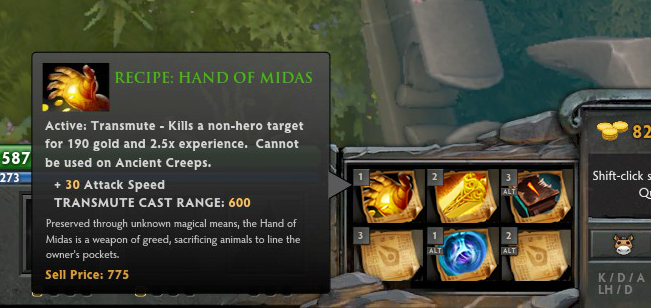
\includegraphics[width=1\textwidth]{recipeseethrucopy}
\caption{My solution}
\end{figure}

\end{document}  
